\documentclass[12pt]{article}

\usepackage{ifpdf}
\usepackage[utf8]{inputenc}
\usepackage[T1]{fontenc}
\usepackage[francais]{babel}
\usepackage{lmodern}
\usepackage{graphicx}
\usepackage[margin=2.5cm]{geometry}
\usepackage{amsmath}
\usepackage{amssymb}
\usepackage{mathrsfs}
\usepackage{hyperref}
\usepackage{braket}
\usepackage{url}
\usepackage{cancel}
\usepackage{units}
\usepackage{array}
\usepackage{url}

\newcommand{\partd}[2]{\frac{\partial #1}{\partial #2}}
\renewcommand{\P}{\mathcal{P}}
\renewcommand\k{k_{\mbox{\tiny{B}}}}
\newcommand{\C}{\mathcal{C}}
\newcommand{\inv}[1]{\frac{1}{#1}}
\newcommand{\var}[1]{\mean{#1 ^2} - \mean{#1} ^2}
\newcommand{\dT}[1]{\frac{\partial #1}{\partial T}}
\newcommand{\efrac}[2]{^{\nicefrac{#1}{#2}}}
\newcommand{\mean}[1]{\left\langle #1 \right\rangle}
\newcommand{\dbmean}[1]{\left\ll #1 \right\gg}
\renewcommand{\d}[1]{\mathrm{d}#1}

\newcommand{\nablaf}{\overrightarrow{\nabla}}
\title{L'allée de Von Karmann pour un obstacle oscillant\\
Cours de physique numérique}

\author{Corentin Cadiou \and Antoine Petit}
\date{}

\begin{document}

\maketitle

\tableofcontents

\section*{Introduction}

	Le passage entre l'écoulement laminaire et la turbulence se fait par des régimes instables ainsi que périodique comme l'allée de Von Karman dans le cas d'un obstacle placé dans un écoulement.
	Ce phénomène qui intervient autant dans les nuages (au voisinage d'une île) que lors du déplacement d'être aquatiques se prête bien à une simulation numérique car l'équation le dirigeant, celle de Navier-Stokes se prête à l'intégration numérique.
	Nous avons, dans le cadre de ce projet, modélisé ce phénomène puis appliqué à un cas particulier, celui d'un objet nageur. Dans ce cas, on observe que les tourbillons induits par l'obstacle peuvent s'inverser, propulsant l'obstacle plutôt que de le freiner.

\section{L'allée de Von Karman}
	
	Le régime de l'écoulement d'un fluide autour d'un obstacle diffère en fonction du nombre de Reynolds associé au fluide et à l'obstacle : à faible Reynolds, l'écoulement est laminaire, à fort nombre de Reynolds l'écoulement est turbulent. Dans le cadre de cette étude, on s'intéresse à un régime intermédiaire, celui de l'allée Von Karman. Dans ce régime, deux tourbillons se forment derr!ère l'obstacle, une perturbation détache l'un des deux, ce qui crée une dépression derrière l'obstacle donnant une vitesse vetricale au second. Le secon tourbillon est à son tour entrainé par le fluide par advection et ainsi de suite.
	
\begin{center}
  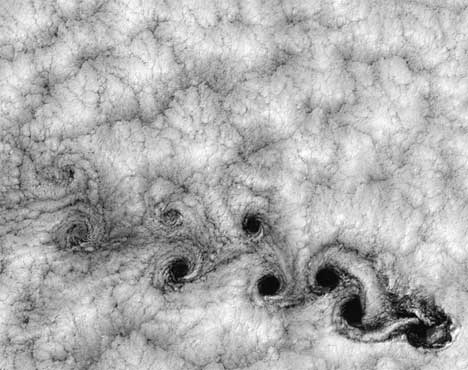
\includegraphics[width=0.6\textwidth]{von-karman-clouds.jpg}
\end{center}
  
	Le phénomène est périodique et on peut montrer par analyse dimensionnelle que la fréquence d'émission des tourbillons est fonction du nombre de Reynolds : $f = \frac{U_0}{D}g(Re)$. Dans le cadre d'un cylindre $\frac{fD}{U_0}=0,198\left (1-\frac{19,7}{Re}\right )$ \cite{Von_Karman}
	
		\subsection{À propos des dimensions du problème}
	
		Notre schéma numérique représente l'équation de Navier-Stokes adimensionnée :

		\begin{equation}
			\partd{\overrightarrow{u}}{t} + (\overrightarrow{u} \cdot 	\nablaf) \overrightarrow{u} = - \nablaf (\phi) + \frac{1}{\mathrm{Re}} \overrightarrow{\Delta} \overrightarrow{u}
			\label{NS}
		\end{equation}
	
		Où $\overrightarrow{u}$ est la vitesse renormalisée par $U_0$ la vitesse du fluide à l'infini,
		les longueurs sont adimensionnées par $L$ la largeur de l'obstacle,
		t est renormalisé par $T_0 = \frac{L}{U_0}$,
		$\phi$ est la pression divisée par $\rho {U_0}^2$ ($\rho$ est la masse volumique du fluide)
		et Re est le nombre de Reynolds : Re = $\frac{\rho L U_0}{\eta}$ ($\eta$ est la viscosité cinématique).
	    
	   
		Les distances et le temps sont bien renormalisés par la donnée de la taille de la grille pour les distances et la condition CFL pour le temps.
	
		\subsection{La force de traînée}

		Des études sur le déplacement des insectes ont montré que si l'obstacle oscille, la force de trainée peut s'inverser et pousser l'objet, nous avons calculer la force de trainée.	
		
		On calcule la force de traînée par intégration du tenseur des contraintes sur un contour carré autour de l'obstacle (soulignons que la force est ici linéique dû au caractère bidimensionnel du modèle) :
	
		\begin{equation}
			\overrightarrow{F_t} = \int_\C [\sigma]\cdot\overrightarrow{\d l} \ \mathrm{où} \ \sigma_{ij} = - p \delta_{ij} + \eta \left(\partd{u_i}{x_j} + \partd{u_j}{x_i}\right)
			\label{trainee}
		\end{equation}
		
		Si on adimensionne \eqref{trainee} comme l'équation de Navier-Stokes \eqref{NS} on obtient :
		\begin{align*}
			\sigma_{ij} 	& = - p \delta_{ij} + \eta \left(\partd{u_i}{x_j} + \partd{u_j}{x_i}\right)\\
						& = \rho U_0^2 \left( - \phi \delta_{ij} + \frac{\eta}{L U_0} \left(\partd{\hat{u_i}}{\hat{x_j}} + \partd{\hat{u_j}}{\hat{x_i}}\right)\right)
        \end{align*}

        Ce qui donne pour la force de trainée :
		\begin{equation}
			\overrightarrow{F_t} = F_0 \int_\C \left[ - \phi \delta_{ij}+ \frac{1}{\mathrm{Re}} \left(\partd{\hat{u_i}}{\hat{x_j}} + \partd{\hat{u_j}}{\hat{x_i}}\right) \right] \cdot \d \hat{l_j} \ \mathrm{où} \ F_0 = \rho U_0^2 L
		\end{equation}
		
	
	
	
	

\section{Le schéma}

	\subsection{Le calcul des champs de vitesses}
		
		Le champ de vitesse est calculé en plusieurs étapes. Tout d'abord on effectue une advection pure au moyen du schéma \eqref{advection} d'ordre 2 en espace. On note $(u,v)$ le champ de vitesse et $(u^*,v*)$ le champ résultant de la première étape.
		
		\begin{equation}
			{u^*}_{i \ j}^{n} = u_{i \ j}^n - {\d t}( u_{ij}^n \frac{u_{i+1 \ j}^n-u_{i-1 \ j}^n}{2 \d x} + v_{i \ j}^{n} \frac{u_{i \ j+1}^n-u_{i \ j-1}^n}{2 \d y}) \\
			\label{advection}
		\end{equation}

		
		On tient ensuite compte de l'obstacle, pour cela, on impose la nullité de la vitesse à l'intérieur de l'obstacle à la fin de l'advection.
		
		Cependant nous n'avons pas tenu compte ici du champ de pression et de la diffusion. On ajoute donc ensuite la contribution de la diffusion à la vitesse au moyen du schéma \eqref{Laplacien} et on note $(u^**,v**)$ le champ résultant de l'étape de diffusion.
		
		\begin{equation}
			{u^{**}}_{i j}^n=	{u^*}_{i \ j}^{n} + 
							\frac{\d t}{\mathrm{Re}} \left(\frac{{u^*}_{i+1 \ j}^n + {u^*}_{i-1 \ j}^n}{{\d x}^2} + \frac{{u^*}_{i \ j+1}^n + {u^*}_{i \ j-1}^n}{{\d y}^2} - \frac{{u^*}_{i \ j}^{n}}{2({\d x}^2 + {\d y}^2)} \right)
			\label{Laplacien}
		\end{equation}
		
		On annule comme précédemment la vitesse dans l'obstacle.
		
		Cependant, lors de ces calculs, on a perdu l'incompressibilité du fluide, afin de garantir l'incompressibilté du fluide, on a recours à une projection de la vitesse. En effet à cette étape, $\overrightarrow{u^{**}}$ vérifie seulement l'équation partielle
		\[ \partd{\overrightarrow{u}}{t} + (\overrightarrow{u} \cdot 	\nablaf) \overrightarrow{u} =  \frac{1}{\mathrm{Re}} \overrightarrow{\Delta} \overrightarrow{u} \],
		c'est-à-dire sans le gradient de la pression, en conséquence, $\overrightarrow{u}$ n'est pas de divergence nulle :
		\begin{align*}
			\nablaf \cdot \overrightarrow{u^{**}} 	& = \nablaf \cdot \overrightarrow{u}	& + &\nablaf \cdot ( [\mathrm{Schéma \ d'advection}] + [\mathrm{Schéma \ de \ difffusion}])\\
													& = 0 								&+ & (\nablaf \cdot \nablaf) \phi & &\\
													& = \Delta \phi & &\\
		\end{align*}
		
		L'idée est donc de calculer la pression via l'inversion de ce laplacien, puis de retrancher le gradient de la pression à ${u^{**}}^n$ pour obtenir $u^{n+1}$. On commence donc par calculer la pression vian l'invesrion du système linéaire induit par le schéma choisi pour le laplacien :
		\[ \phi = L^{-1}(\nablaf \cdot \overrightarrow{u^{**}})\]
		
		Où $L$ est la matrice du schéma du laplacien.
		
		Ensuite on calcule $(u^{n+1},v^{n+1})$ par projection \eqref{proj}.
		
		\begin{equation}
			u^{n+1}_{i \ j}={u^{**}}_{i \ j}^{n+1} - \frac{\phi^n_{i+1 \ j}-\phi^n_{i-1 \ j}}{2\d x}
			\label{proj}
		\end{equation}
		\[	v^{n+1}_{i \ j}={v^{**}}_{i \ j}^{n+1} - \frac{\phi^n_{i \ j+1}-\phi^n_{i \ j-1}}{2\d y} \]

		La vitesse dans l'obstacle n'est pas parfaitement nulle, mais ceci est nécessaire car si l'on faisait comme précédemment, on perdrait l'incompressibilité du fluide. Il y a donc une vitesse résiduelle sur le bord de l'obstacle, en conséquence le schéma est d'ordre 1 en espace et en temps.
		
		Nous reviendrons plus tard sur les améliorations et les modifications que nous avons apporté à ce schéma initial.		
		
		\subsubsection{La condition CFL}
		
			Afin que $u_max \d t < \max(\d x, \d y)$, on contrôle le pas de temps avec cette condition afin de ne pas perdre en précision lors des itérations.
		
		
	\subsection{Les conditions aux limites}
		
		\subsubsection{Au bord}
			Afin de pouvoir calculer les dérivées sur toute la zone de simulation, on rajoute autour de la zone "physique" un contour de points dits fantômes, on fixe en ces points la valeur afin de garantir des conditions au limites : 
			\begin{itemize}
				\item À gauche : $(u,v) = (U_0,0)$ afin de simuler l'écoulement.
				\item Sur En haut et en bas et à droite, on recopie les valeurs, ce n'est pas très gênant car les points sont très vite advectés en dehors de la simulation
			\end{itemize}
		
		\subsubsection{Sur l'obstacle}

			Comme vu précédemment, l'obstacle est modélisé par une zone de vitesse nulle, c'est pour cela qu'à chaque calcul de la vitesse, on annule la vitesse dans l'obstacle afin de maintenir la condition. Nous avons modifié cette condition dans la suite pour permetrre à l'obstacle de bouger.

	\subsection{La visualisation des tourbillons}
	
		La technique choisie pour observer les vortex est celle de l'advection par le champ de vitesse d'un traceur : Pour cela nous avons essayé deux solutions différentes : une première consistait à insérer un colorant à une concentration 1 en divers points à la gauche de l'obstacle, puis à le laisser transporter par le champ de vitesse. La seconde consistait à colorer l'ensemble de la simulation à part l'obstacle qui absorbait le colorant (on annule la valeur de la concentration de colorant sur l'obstacle), dans ce cas-ci les tourbillons sont visualisé par le déficit local de colorant.
		
		Cependant ces technique manquait de précision du fait de la diffusion numérique due au schéma d'advection, rapidement on ne distinguait plus les zones très colorés, c'est pourquoi nous avons utilisé un autre schéma pour l'advection du colorant basé sur la méthode dite \emph{BFECC}.
		
	\subsection{\emph{Back and forth error compensation and correction methods (BFECC)}}
		Cette méthode décrite par Kim \cite{Advect} et Dupont \cite{BFECC} consiste à appliquer successivement trois fois le schéma d'advection en aller retour pour compenser le terme linéaire de dispersion numérique.
		
		Si on nomme $A(\overrightarrow{v},X)$ l'opérateur d'advection par $\overrightarrow{v}$ du champ $X$, le schéma de la \emph{BFECC} est le suivant :
		\begin{align*}
  			X_1 &	= A(\overrightarrow{v},X^n) \\
			X_2	&	= A(-\overrightarrow{v},X_1)\\
			X^{n+1}&	= A(\overrightarrow{v},X^n-\alpha(X^n-X_2))
		\end{align*}	
		
		\begin{figure}[htbp]
		\begin{center}
			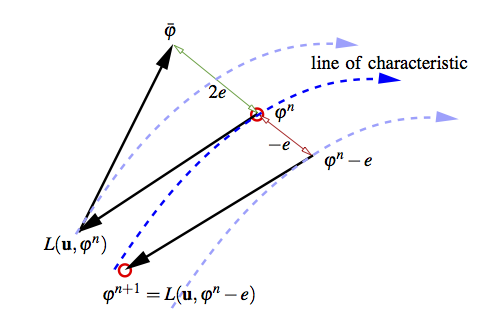
\includegraphics[width=0.7 \textwidth]{explain_BFECC.png}
			\caption{L'idée de la méthode \emph{BFECC}, l'erreur $e$ est retrancher ce qui fait passer le schéma à l'ordre 2 \cite{Advect}}
		\end{center}
		\end{figure}				
		
		La méthode est du deuxième ordre si $\alpha = \frac{1}{2} $ car l'erreur induite par l'advection d'ordre 1 est compensée par le terme ajouté dans la troisième advection.
		
		Cette méthode est très efficace comme on peut le constater sur les figures \ref{Comparaison}, on remarque que l'on gagne en précision sur la définition des tourbillons, cependant cette méthode a plusieurs défauts. Pour commencer nous avons eu des problèmes d'instabilité lors de sa mise en place car les conditions aux limites du colorant entrainait une croissance exponentielle de la concentration à la frontière du domaine \ref{instabilite}.
		
		\begin{figure}[htbp]
			\begin{center}
			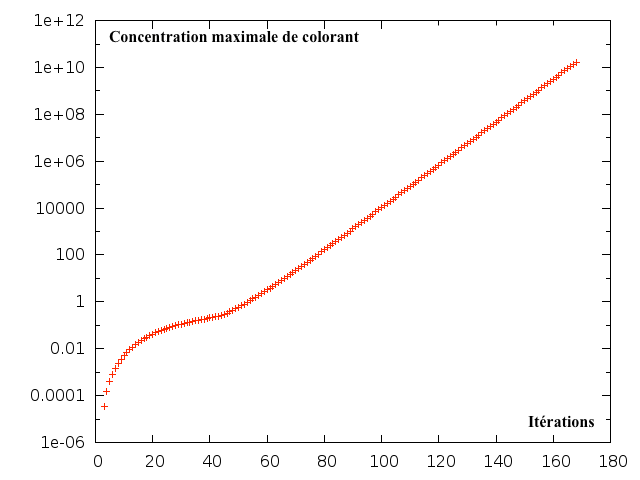
\includegraphics[width=0.7 \textwidth]{instabilite.png}
			\caption{Maximum de la concentration du colorant en fonction du nombre d'itérations}
			\label{instabilite}
			\end{center}
		\end{figure}
		
		Un autre désavantage de la \emph{BFECC} dans sa version d'ordre 2 est l'apparition d'un comportement dispersif. Le schéma présente alors plus d'inconvénients que d'avantages : en effet les tourbillons se désagrègent plutôt que d'être advecté. La solution que nous avons choisie est d'utiliser $\alpha < 0,5$, par exemple $\alpha = 0,25$. En effet avec un coefficient plus faible on réduit l'erreur tout en maintenant un schéma diffusif qui évite la dispersion.
		
		\begin{figure}[htbp]
		\begin{center}
			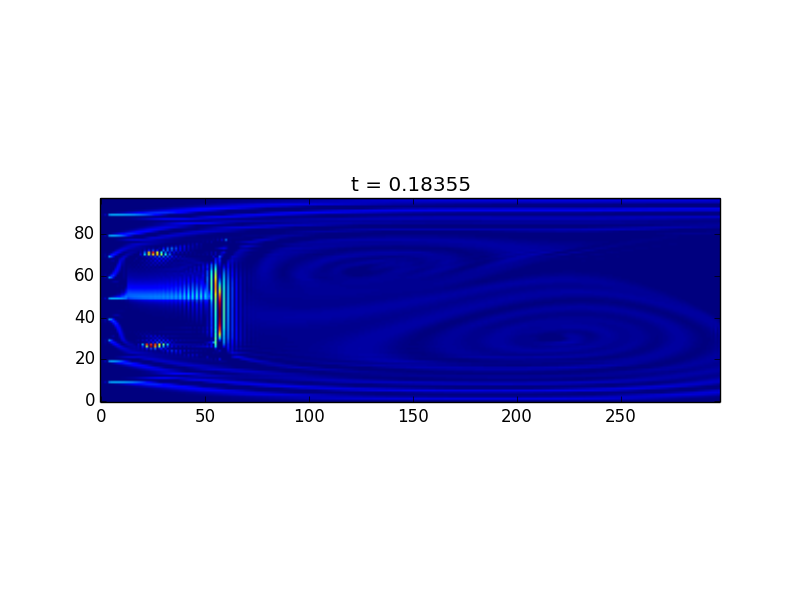
\includegraphics[width=0.8 \textwidth]{BFECC.png}
			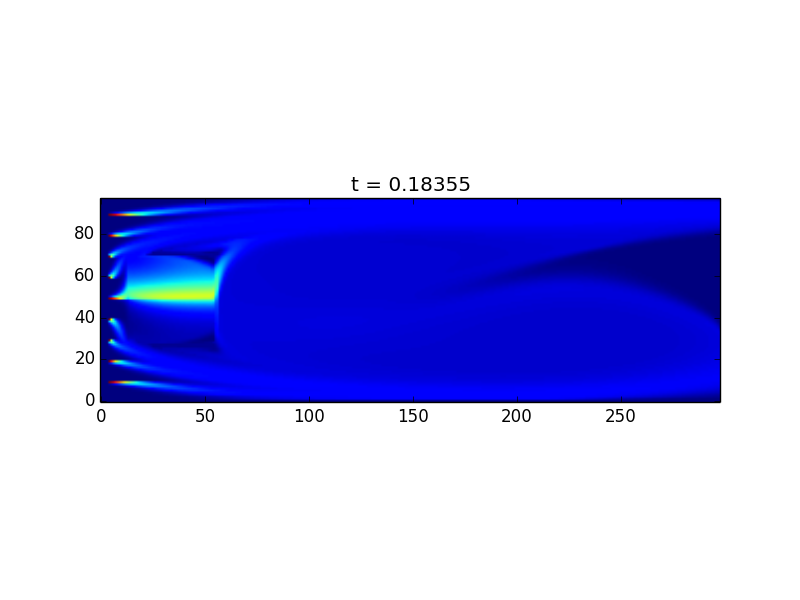
\includegraphics[width=0.8 \textwidth]{NO-BFECC.png}
			\caption{Deux simulations aux même temps avec et sans \emph{BFECC}. Le colorant dans l'obstacle est dû à une erreur de code fixée ensuite}
			\label{Comparaison}
		\end{center}
		\end{figure}
		
		Sur la figure \ref{Comparaison}, on voit à la fois les avantages et inconvénients de la méthode \emph{BFECC}, si cette dernière offre une plus grande précision, la présence d'artefacts dispersif est fort gênante. 
	
	\subsection{La pénalisation}

		Les mouvements de l'obstacle sont saccadés. En effet même si le mouvement est sinusoïdal, l'obstacle peut seulement bouger de case en case. Par conséquent on observait sur le tracé de la traînée des discontiunités au changement de case. Pour éviter ces discontinuités, nous avons appliqué une méthode de pénalisation sur l'obstacle, en effet la discontinuité induite par le mouvement de l'obstacle est celle répercutée par la mise à zéro de la vitesse dans l'obstacle. L'idée est de rendre "perméable" la frontière de l'obstacle en atténuant progressivement la vitesse dans celui-ci. Le schéma utilisé est comparable à une forme d'effet de peau \eqref{penalisation}. 
		
		\begin{equation}
			\forall x \in \mathcal{O}bs, \ \ \
			u^{n+1}(x)= u^n_{obs}(x) + (u^n(x)-u^n_{obs}(x))\mathrm{e}^{-\alpha\d t}
			\label{penalisation}
		\end{equation}
		
		La vitesse décroit donc exponentiellement dans l'obstacle avec une constante de temps $\tau= \alpha^{-1}$. Le cas $u(x\in \mathcal{O}bs)=u_{obs}$ correspond au cas limite $\alpha = +\infty$.
		
		\begin{figure}[htbp]
		\begin{center}
			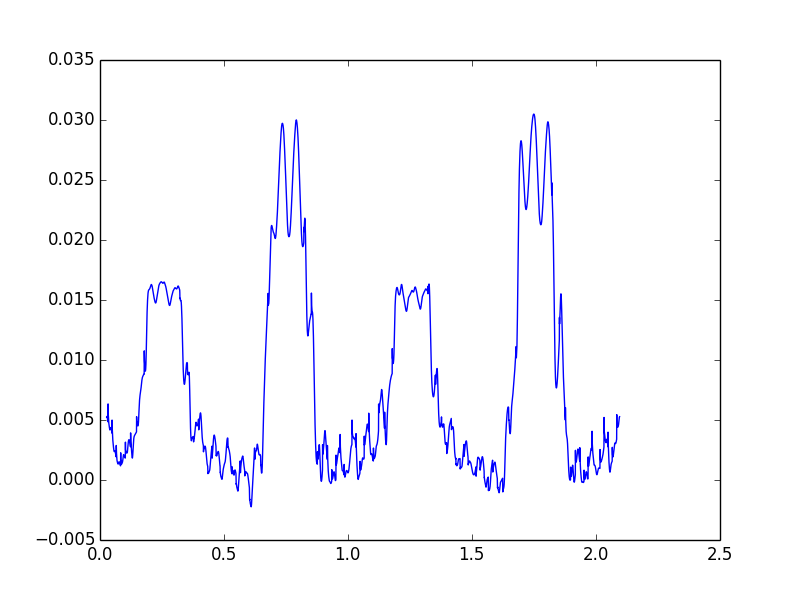
\includegraphics[width=0.7 \textwidth]{drag_degueu.png}
			\caption{La force de traînée sans pénalistation de la vitesse dans l'obstacle.}
		\end{center}
		\end{figure}


\section{Le code}

	\subsection{Les options}
		
		Elles permettent de donner les caractéristiques de la simulation que l'on souhaite effectuer :\\
			\begin{table}[htbp]

			\begin{tabular}{|l | p{7cm}| l |}
				\hline
				\textbf{Nom} & \textbf{Description} & \textbf{Arguments}\\
                \hline
				\hline
				\-\-hash & Utilise une table de hashage & \\
				\hline
				- -BFECC & Utiliser la méthode \emph{BFECC} & Booléen\\
				\hline
				- -tracer & Visualiser par injections de traceurs & Par défaut 10\\
				\hline
				- -behind & Obstacle absorbant le colorant & \\
				\hline
				- -Re & Nombre de Reynolds &  Par défaut 1e4\\
				\hline
				- -nx, - -ny & Taille de la grille &  Par défaut 150, 80\\
				\hline
				- -ox & Position de l'obstacle (à gauche) &\\
				\hline
				- -parallel & Utiliser le calcul parallèle pour le plot& Par défaut False\\
				\hline
				- -max parallel & Utiliser le calcul parallèle pour le plot & \\
				\hline
				- -speed & Vitesse du fluide & Par défaut 1 \\
				\hline
				- -sinus & On anime l'objet d'un mouvement sinusoïdal vertical & Par défaut freq=0 amp=0\\
				\hline
				- -rect & L'obstacle est un rectangle & Par défaut (width,height) = (10,10)\\
				\hline
				- -circle & L'obstacle est un cercle & Écrase l'option rectangle\\
				\hline
				- -movie & La sortie donne la série d'images  & \\
				\hline
				- -alpha & Gère le coefficient de pénalisation & Par défaut 10 000\\
				\hline
				- -niter & Nombre d'itérations de la simulation & Par défaut 10 000\\
				\hline
			\end{tabular}
			\caption{Les différentes options de la simulation}	
			\end{table}
			
	\subsection{Le calcul du Drag}
	
		Comme expliqué dans la section précédente, on calcule la traînée en intégrant le tenseur des contraintes sur un contour autour de l'objet, pour cela on calcule la Jacobienne aux points du contour choisi, puis on calcule $\sigma$ et on somme l'intégrale numériquement. On trace ensuite cette valeur en fonction du temps
		
		
	\subsection{L'obstacle oscillant}
		
    Afin d'inverser la traînée, nous avons dû calculer une fonction
permettant de déplacer l'obstacle. Une première permettait de faire
bouger l'obstacle verticalement, de manière sinusoïdale. Il suffisait
de varier la position $oy$ du rectangle.

Pour simplifier la démarche pour effectuer des rotations,
nous avons ensuite créé une classe python décrivant l'obstacle et
donnant accès à des méthodes comme par exemple la position du point de
rotation et permettant d'éffectuer des améliorations de performances
lors de l'exploration de tous les points contenus dans l'obstacle.

Pour modéliser la rotation de l'obstacle, nous avons décidé d'itérer
sur tous les points de l'obstacle (grâce à un itérateur que nous avons
écrit) et d'appliquer une matrice de rotation dépendant de la position
du point de pivot, du temps, de la fréquence et de l'amplitude de
l'oscillation. Notons $M$ le masque, $O$
l'ensemble des points de l'obstacle et $R$ la rotation d'angle $\theta$.

Notre masque est l'ensemble :
\[ M = \left\lbrace (x,y) \in \mathbb{Z}^2 / R^{-1}(x,y)
  \in O \right\rbrace \]

Une fois cette ensemble construit, il suffit de parcourir tous les
éléments de $M$ et d'appliquer le masque au champ de vitesse à
l'instant $n+1$, noté $\phi^{n+1}$ selon la pénalisation (définie par
une fonction $p(x,y)$) : 
\[ \forall (x,y)\in M, \phi^{n+1}(x,y) = p(\phi^{n}(x,y)) \] 
		 
	\subsection{Optimisations du code}
		Dans un premier temps, des outils de détection des parties
inutilisées du code ont été utilisés (\emph{pyflakes} pour supprimer les
fonctions et les imports inutilisés et \emph{coverage} pour détecter les
variables inutilisées).\\
L'étape suivante a été de tenter de remplacer toutes les boucles for
par la structure plus naturelle en python 2 de compréhension de liste
, ceci pour gagner environ $5-10\%$:

\begin{minipage}[t]{0.5\textwidth}
\paragraph{Classique  : $t_{exec} = 3.3s$}

\begin{verbatim}
import numpy as np
f = lambda x : np.sin(2*np.pi*x)
l = []

for i in xrange(0, 1000000):
    l.append(f(i))
\end{verbatim}
\end{minipage}
\begin{minipage}[t]{0.5\textwidth}
\paragraph{Compréhension de liste : $t_{exec} = 3.1s$}

\begin{verbatim}
import numpy as np
f = lambda x : np.sin(2*np.pi*x)

l = [f(i) for i in xrange(0, 1000000)]
\end{verbatim}
\end{minipage}

On constate de plus un gain en concision.
\subsubsection{Le calcul parallèle}
        La librairie utilisée pour afficher les images est
matplotlib.pyplot. Cependant, une analyse des appels de fonction a
montré que l'affichage occupait un temps non négligeable lors de
l'éxecution du programme, comme le montre la figure \ref{call}.
\begin{figure}
  \begin{center}
    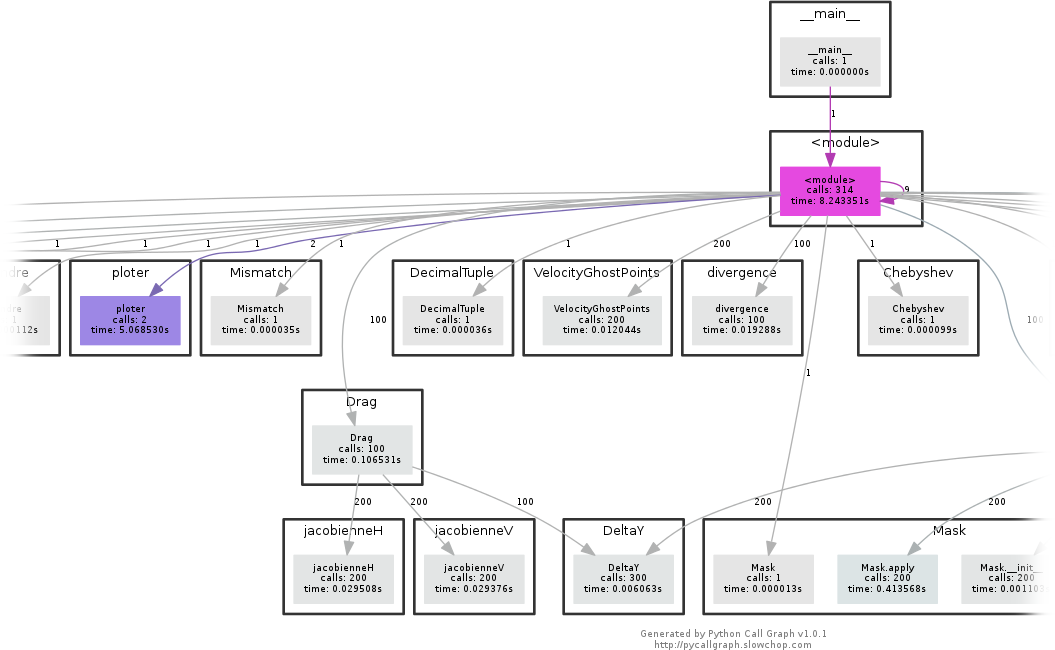
\includegraphics[width=0.9\textwidth]{pycallgraph.png}
    \caption{Extrait du fichier généré par l'outil pycallgraph. On
      constate que l'appel de la fonction ``ploter'' occupe $5.06$s
      sur $8.24$s d'exécution totale. On notera que pour ce test, on a
      choisi une fréquence d'affichage très régulière.}
    \label{call}
  \end{center}
\end{figure}
Pour optimiser l'exécution du programme, un système de calcul en
parallèle a été implémenté (\emph{via} le module PP). Dans un premier
temps, l'affichage dans une fenêtre graphique a été supprimé pour
imprimer la sortie dans un fichier. Grâce à cela, il a été possible de
faire créer les images par un \emph{thread} indépendant.

Dans un second temps, les calculs ont été réalisés en parallèle
aussi. L'optimisation s'est focalisée sur la partie qui calcule les
matrices d'advections. Une première phase d'optimisation a consisté à
créer un ``table de hashage'' dans laquelle toutes les matrices
précalculées sont stockées. Une telle table est un tableau associatif
qui a un champ de vitesse (identifié par son ``hash'' associe un
ensemble de matrices). Ainsi, pendant l'éxecution d'une BFECC,
on calcule l'ensemble des matrices associées au champ de vitesse
$\phi$ noté $E[\phi]$. On effectue une étape d'advection avec $\phi$
puis une autre avec $-\phi$. Enfin, on corrige l'erreur éstimée en
et on refait une étape d'avection avec comme champ $\phi$. Il est donc
dommage de devoir recalculer les matrices déjà calculées plus haut,
puisqu'elles sont déjà dans $E[\phi]$.\\
Le calcul en parallèle intervient justement dans le calcul de ces
matrices. En notant toujours $\phi$ le champ de vecteur, qu'on peut
considérer comme deux matrices $U$ et $V$ (ses composantes selon $x$
et $y$), l'advection nécessite de calculer (à des constantes près): 
\begin{align*}
  \left| U \right | & &  1 - \left| U \right | & &(1)\\
  \left| V \right | & &  1 - \left| V \right | & &(2)\\
  \textrm{sign}\left( \textrm{sign}(U+1)\right) & &   1 -
  \textrm{sign}\left( \textrm{sign}(U+1)\right) & &(3)\\
  \textrm{sign}\left( \textrm{sign}(V+1)\right) & &   1 -
  \textrm{sign}\left( \textrm{sign}(V+1)\right) & &(4)
\end{align*} 
Il faut ensuite calculer des produits de matrices. Ce genre de calcul
peut très facilement être effectué en parallèle et c'est ce qui a été
réalisé.
 
Pour mesurer l'optimisation ainsi crée, des mesures de temps
d'éxecution du code sur un nombre précis d'itérations a été
réalisé. Les résultats sont présentés dans le tableau
\ref{optimisation}.

On constate que le calcul en parallèle est surtout utile pour
l'affichage. Sur un ordinateur multi-coeur, l'ajout du parallelisme a
permis d'améliorer de $20$ à $40\%$ les performances.\\
Pour être encore plus fin, il convient de discuter des domaines dans
lesquels le mode ``parallèle'' et le mode ``tout-parallèle'' sont les
meilleurs. On se réferera pour cela au tableau
\ref{optimisation_parallel}. Dans notre cas, les simulations ont été
effectuées sur des grilles de l'ordre de grandeur de 100 par 100. On a
donc plutôt utilisé l'option ``parallèle''.

\begin{table}
  \begin{center}
    \begin{tabular}{|c|c|c|c|c|}
      \hline
      Itérations & Taux de rafraîchissement& Normal & Parallèle &
      Tout parallèle \\
      \hline
      1000&	50&	25&	\textbf{16}&	22\\
      100&	10&	8&	\textbf{5}&	6\\
      2000&	100&	35&	\textbf{27}&	39\\
      1000&	100&	16&	\textbf{11}&	17\\
      500&	10&	32&	\textbf{19}&	21 \\
      \hline
    \end{tabular}
    \caption{Tableaux présentants les temps d'éxécution. Les taux de
      rafraîchissement sont en itérations par image. Les temps
      d'éxecution sont en seconde. Les colonnes ``Normal'' (pas de calcul
      parallèle), ``Parallèle'' (affichage dans un \emph{thread}
      indépendant) et ``Tout parallèle'' (affichage et certains
      calculs dans des \emph{threads} indépendants).}
    \label{optimisation}
  \end{center}
\end{table}
\begin{table}
  \begin{center}
    \begin{tabular}{|c|c|c|c|c|}
      \hline
      Taille de la grille&	Parallèle&	Tout parallèle& $\Delta$\\	
      \hline
      100&	2.801&	3.018&	0.93\\
      200&	4.51&	4.091&	1.10\\
      300&	8.593&	7.096&	1.21\\
      400&	15.481&	13.234&	1.17\\
      \hline
    \end{tabular}
    \caption{On a noté $\Delta = \frac{t_{\mathrm{exec,tout
            parallel}}}{t_{\mathrm{exec,parallel}}}$. Tableau de temps
      d'exécution en fonction du parallélisme utilisé. On
      constate que pour une grande grille, le calcul tout en parallèle
      est plus intéressant. Pour des grilles de la taille de celles
      utilisées (100*100), ce n'est pas rentable et il vaut mieux ne
      mettre en parallèle que l'impression des images.}
    \label{optimisation_parallel}
  \end{center}
\end{table}
		 
\section{Analyse des résultats}

	\subsection{L'allée de Von Karman}
	
		On observe bien l'instabilité, tant pour un obstacle rectangulaire que pour un obstacle circulaire. Bien que l'apparition de l'allée soit plus longue dans le cas circulaire car l'obstacle est mieux profilé. Il faut prendre garde à prendre un espace d'étude suffisamment grand pour éviter que l'allée ne sorte par un des côtés car ensuite elle y reste bloquée.
		
		\begin{figure}[htbp]\begin{center}
			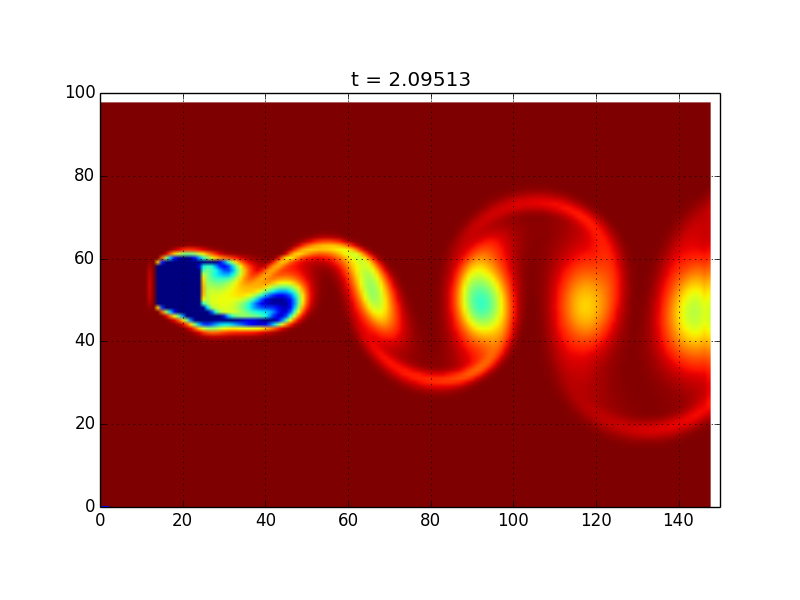
\includegraphics[width=0.8 \textwidth]{VK_pas_mal.png}
			\caption{Un exemple de résultat pour le modèle étudié}
			\label{VK}
		\end{center}\end{figure}	
		
	
	\subsection{La force de trainée, application à l'obstacle oscillant}
	
		Grâce à la méthode de pénalisation, on obtient une courbe
        régulière pour la traînée. Dans le cas d'un obstacle
        oscillant, pour une certaine gamme de fréquences et
        d'amplitudes, on observe que la trainée peut devenir négative,
        nous avons donc calculé $W_t= \int F_t U_0\d t$, le travail
        dans le référentiel du fluide de la force de traînée. Dans
        certaines gammes d'amplitudes et de fréquences, le travail est
        moteur \ref{Wamp}. De plus, pour $ \theta_0 \leq 0,09$, si on
        trace $W_t^{-1}$ le graphe est une droite
        \ref{regressinvers}. On en déduit que pour les petites
        amplitudes, $W_t \propto \theta_0^{-1}$ et est positif, ce qui
        est cohérent . 
		
		\begin{figure}[htbp]\begin{center}
			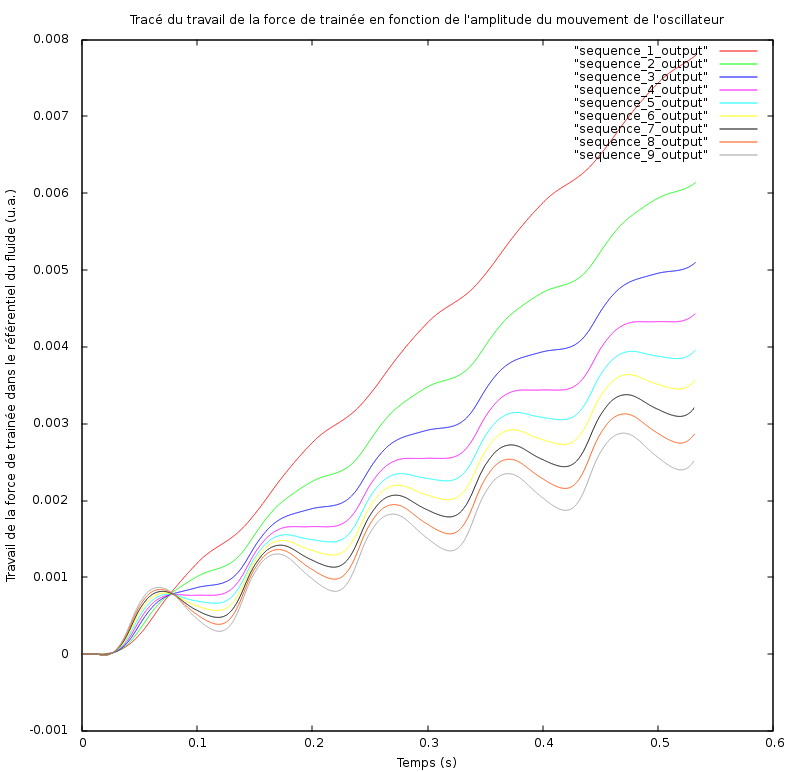
\includegraphics[width=0.9 \textwidth]{9courbes.png}
			\caption{$W_t$ en fonction de l'amplitude pour différentes
              fréquences (les amplitudes vont de 0.001\degre à 0.009\degre par
              ordre croissant)}
			\label{multiW}
		\end{center}\end{figure}				
		
		\begin{figure}[htbp]\begin{center}
			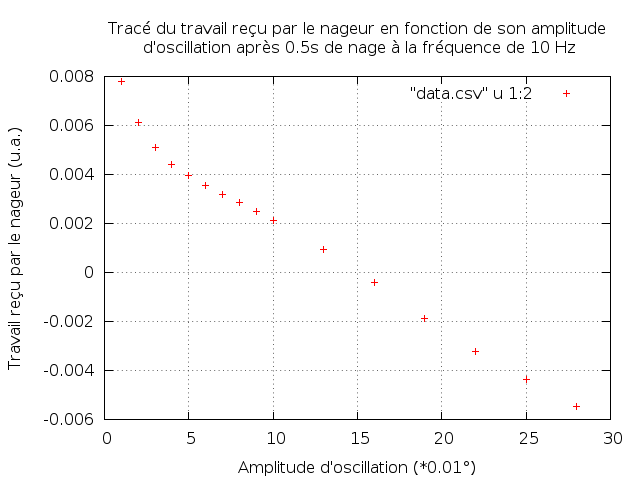
\includegraphics[width=0.9 \textwidth]{bcp_points.png}
			\caption{$W_t^{-1}$ au bout de 2000 itérations à la fréquence en fonction de l'amplitude}
			\label{Wamp}
		\end{center}\end{figure}
		
		\begin{figure}[htbp]\begin{center}
			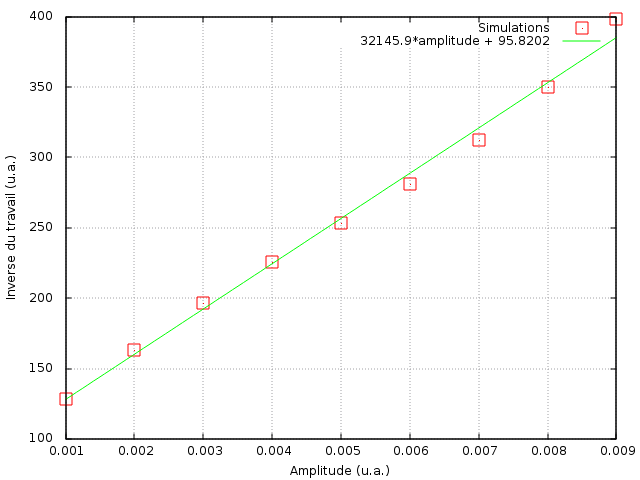
\includegraphics[width=0.7 \textwidth]{9_courbes_extraites.png}
			\caption{Régression linéaire de l'inverse du travail en fonction de l'amplitude dans les mêmes conditions que dans \ref{Wamp}}
			\label{regressinvers}
		\end{center}\end{figure}
		
		
\section*{Conclusion}
	Notre modèle rend effectivement compte de la propulsion chez les têtards par exemple, en effet, l'obstacle "nageur" peut remonter le courant si il oscille avec une amplitude suffisante ou une fréquence suffisament élevée, on re trouve également des résultats qui semblent cohérents comme l'inverse proportionnalité du travail et de l'amplitude pour les petites perturbations.
	Le schéma est consistant et le code est en partie optimisé, ce qui a facilité le calcul de nombreuses simulations.
	Nous aurions aimé faire une étude plus systématique et plus théorique de la force de traînée (évolution en fonction de Re, de la fréquence d'oscillation, taille de l'obstacle,...) et également travailler sur des simulations plus grandes (et donc impliquant un plus grand temps de calcul afin d'essayer de retrouver l'expression de la fréquence d'émission des tourbillons.
	
	
	
	\pagebreak
\bibliographystyle{plain}
\bibliography{Biblio.bib}
	
\end{document}